\documentclass[aspectratio=169,11pt]{beamer}
\usepackage{booktabs,tabularx,array,amsmath,pgfplots}
\pgfplotsset{compat=1.18}
\definecolor{navy}{HTML}{20364C}
\definecolor{teal}{HTML}{147D92}
\setbeamercolor{normal text}{fg=navy,bg=white}
\setbeamercolor{structure}{fg=teal}
\setbeamercolor{frametitle}{fg=navy}
\setbeamerfont{frametitle}{size=\Large,series=\bfseries}
\setbeamertemplate{navigation symbols}{}
\setbeamertemplate{footline}{\hfill{\color{gray}\scriptsize\insertframenumber/\inserttotalframenumber}\hspace{.5cm}\vspace{.15cm}}
\setbeamersize{text margin left=.7cm,text margin right=.7cm}
\setlength{\parskip}{5pt}
\setlength{\parindent}{0pt}
\emergencystretch=1.5em
\setbeamertemplate{itemize item}{\color{teal}\small$\bullet$}
\setlength{\tabcolsep}{4pt}
\newcommand{\src}[1]{\par\vfill{\fontsize{7}{9}\selectfont\color{gray}#1\par}}
\title{PyTorch/GPU Reachability Experiments Since the Previous Presentation}
\date{September 29, 2026}
\begin{document}

% Slide 1
\begin{frame}[t]{PyTorch / GPU Reachability}
\relax
\relax
\vspace{0.35cm}{\LARGE\bfseries Experimental progress since the previous presentation}\par{}
\vspace{0.45cm}{\large QUAD, ARCH-COMP, and four-way comparisons of time and width}\par{}
\vspace{0.65cm}Ours \quad Huan \quad Xiangru \quad Native Flow*\par{}
\vspace{0.4cm}September 29, 2026\par{}
\vfill Starting point: the 29-slide presentation of September 23, 2026.\par{}
All statuses come from saved evidence; no experiments were resumed to prepare this deck.
\src{S00; latest native QUAD snapshot: September 29, 20:19:53 China time.}
\end{frame}

% Slide 2
\begin{frame}[t]{Main results from this phase}
\relax
\relax
\begin{itemize}
\item \textbf{Broader coverage: 14 official configurations.} Seven completed in all four methods, each with five measured runs.
\item \textbf{Our corrected P3 completed the full QUAD task.} All 1024 partitions were accepted through 1000 steps; corrected P2 had a common prefix of 799 steps.
\item \textbf{Full P3 runtime fell by 51.36\%.} It dropped from 52.56 to 25.56 minutes with identical saved ranges and final states.
\item \textbf{Width interpretation changed materially.} The old native ACC reference has an enclosure failure; Unicycle still has a substantial width gap; Airplane now reaches a real NN property stop.
\end{itemize}
\src{S01, S03–S06, S11–S12. The new QUAD candidate has not yet passed a full benchmark regression.}
\end{frame}

% Slide 3
\begin{frame}[t]{What the project computes}
\relax
\relax
Given a set of initial states and a neural-network controller, we enclose every possible trajectory.\par{}
\vspace{0.2cm}
{\small\renewcommand{\arraystretch}{1.18}\noindent\begin{tabularx}{\linewidth}{@{}p{3cm}X@{}}\toprule
\textbf{Stage} & \textbf{Role}\\\midrule
NN bounds & Compute affine lower and upper bounds on the controller output over the current state set.\\
Dynamics propagation & Propagate the state using Taylor-model polynomials and interval remainders.\\
Validation and SR & Check inclusion of new remainders; SR retains cross-step error dependence.\\
Ranges and properties & Export endpoint and full-step tube bounds and evaluate the specified property.\\
\bottomrule\end{tabularx}\par{}}\vspace{0.25cm}Runtime measures cost; width measures conservatism. We must also check set inclusion and the portion of the task completed.
\src{S01; the main comparisons include the closed-loop NN. Offline replays and one-step diagnostics are labeled separately.}
\end{frame}

% Slide 4
\begin{frame}[t]{Frozen revisions and explicit entry points}
\relax
\relax
{\small\renewcommand{\arraystretch}{1.18}\noindent\begin{tabularx}{\linewidth}{@{}p{2.2cm}p{5.8cm}X@{}}\toprule
\textbf{Method} & \textbf{Revision / implementation} & \textbf{Interpretation here}\\\midrule
Ours & Huan-derived worktree fff9d0f; separate P2/P3 entry points & Not assumed merged into our public repository.\\
Huan & flowstar-gpu d5f0b68 & Default mode differs from suite strict mode.\\
Xiangru & CROWN-Reach\_\allowbreak Development 1c16d4e & Integrated driver, models, and GPU kernels.\\
Native Flow* & C++ library in CROWN-Reach 7b90f30 & Fixed-step wrapper; repair labeled separately.\\
\bottomrule\end{tabularx}\par{}}\vspace{0.2cm}{\small All three GPU suite rows use Xiangru's driver with strict dynamics and box/same-slope/RPC32. Independent pendulum defaults use hybrid/parity.\par{} Huan and Xiangru share 27/29 core Python files and the same CUDA math; 13 comparable range files are byte-identical.}
\src{S01. These comparisons do not characterize every author branch or later revision; exact repository identities are in the data bundle.}
\end{frame}

% Slide 5
\begin{frame}[t]{How to read runtime and width}
\relax
\relax
{\small\renewcommand{\arraystretch}{1.18}\noindent\begin{tabularx}{\linewidth}{@{}p{3cm}X@{}}\toprule
\textbf{Measure} & \textbf{Definition and scope}\\\midrule
Measured runtime & Wall time of a fresh process, including imports, cached extension loading, NN initialization, and solve; median of five runs; excludes first compilation.\\
Single diagnostic & May include observation, checkpoints, and audits; time before failure is never used as a full-task speed denominator.\\
Per-partition width & Upper minus lower bound for one partition, coordinate, and time; report mean or maximum.\\
Global hull width & Largest upper minus smallest lower bound over partitions: \(W_{\rm hull}=\max_b u_b-\min_b l_b\).\\
Width ratio & GPU / native, only over a common valid prefix. Zero or tiny denominators are identified separately.\\
\bottomrule\end{tabularx}\par{}}\vspace{0.2cm}An endpoint is the end of a step; a tube covers the whole step. Mean partition width and global hull width are different measures.
\src{S01; runs shared a V100 node rather than an exclusive machine.}
\end{frame}

% Slide 6
\begin{frame}[t]{Coverage of the 14 official configurations}
\relax
\relax
{\small\renewcommand{\arraystretch}{1.18}\noindent\begin{tabularx}{\linewidth}{@{}p{2.7cm}p{6.0cm}X@{}}\toprule
\textbf{Group} & \textbf{Configurations} & \textbf{Outcome}\\\midrule
Four-way complete: 7 & Attitude, Unicycle, two heterogeneous TORA variants, NAV robust, Single Pendulum, ACC* & Five full runtimes per method; a defect in the ACC reference was found later.\\
Partial: 4 & DP less robust, NAV standard, CartPole, TORA homogeneous & Native timeouts or GPU rejections; retain common prefixes.\\
Property stops: 2 & DP more robust, Airplane & Stop semantics and actual model must be checked; Airplane later ran with a GPU NN connection.\\
Targeted repair: 1 & QUAD & Earlier numerical failure or resource stop; P3 now completes 1000 steps.\\
\bottomrule\end{tabularx}\par{}}\vspace{0.3cm}VCAS provides an NN service/simulation, but no comparable C++ reachability entry point was found; it is not counted as a fifteenth case.
\src{S01, S11. Completion of a run does not by itself establish a full rigorous NNCS proof.}
\end{frame}

% Slide 7
\begin{frame}[t]{Seven complete cases: four-way runtime}
\relax
\relax
{\small\setlength{\tabcolsep}{3.2pt}\renewcommand{\arraystretch}{1.18}
\noindent\begin{tabular*}{\linewidth}{@{\extracolsep{\fill}}lrrrr@{}}\toprule
\textbf{Benchmark} & \textbf{Ours} & \textbf{Huan} & \textbf{Xiangru} & \textbf{Flow*}\\ \midrule
Attitude & 7.121 & 6.990 & 7.028 & 6.315\\
Unicycle & 6.909 & 9.796 & 9.581 & 10.722\\
TORA ReLU/tanh & 7.685 & 12.421 & 12.332 & 8.632\\
TORA sigmoid & 8.208 & 13.165 & 13.274 & 9.098\\
NAV robust & 9.730 & 14.646 & 14.814 & 68.164\\
Single Pendulum & 5.176 & 5.597 & 5.618 & 4.908\\
ACC* & 7.793 & 8.035 & 7.960 & 8.259\\
\bottomrule\end{tabular*}\par{}}\vspace{0.12cm}{\small Seconds; median of five complete fresh-process runs. Ours is about 7.01\(\times\) faster on NAV robust and 1.55\(\times\) faster on Unicycle.\par{}Attitude and Single Pendulum are still slower than native. ACC* retains only the historical execution time.}
\src{S01. The old native ACC* reference was later shown to miss reachable states; it cannot certify accuracy against a correct reference.}
\end{frame}

% Slide 8
\begin{frame}[t]{Complete cases: worst width ratio over time}
\relax
\relax
{\small\setlength{\tabcolsep}{3.2pt}\renewcommand{\arraystretch}{1.18}
\noindent\begin{tabular*}{\linewidth}{@{\extracolsep{\fill}}lrrrr@{}}\toprule
\textbf{Benchmark} & \textbf{Huan local} & \textbf{Xiangru local} & \textbf{Ours local} & \textbf{Ours global}\\ \midrule
Attitude & 1.1456 & 1.1456 & 1.1456 & 1.1456\\
Unicycle & 3.4435 & 3.4435 & 3.4994 & 3.4994\\
TORA ReLU/tanh & 1.0077 & 1.0077 & 1.0081 & 1.0081\\
TORA sigmoid & 1.0107 & 1.0107 & 1.0107 & 1.0107\\
NAV robust & 1.0388 & 1.0388 & 1.0465 & 1.0123\\
Single Pendulum & 1.0921 & 1.0921 & 1.0581 & 1.0581\\
\bottomrule\end{tabular*}\par{}}\vspace{0.3cm}Each entry is the worst ratio to native across common times, coordinates, and endpoint/tube views.\par{}Heterogeneous TORA and NAV robust are close to native. The roughly 3.50\(\times\) Unicycle gap reflects real width, not rounding in the last digit.
\src{S01. Local means per partition; global means the union hull. Old ACC ratios are corrected separately and excluded from the accuracy ranking.}
\end{frame}

% Slide 9
\begin{frame}[t]{Unicycle: faster, but a wider final range}
\relax
\relax
{\small\setlength{\tabcolsep}{3.2pt}\renewcommand{\arraystretch}{1.18}
\noindent\begin{tabular*}{\linewidth}{@{\extracolsep{\fill}}lrrrr@{}}\toprule
\textbf{Endpoint at T=10} & \textbf{Flow*} & \textbf{Huan} & \textbf{Xiangru} & \textbf{Ours}\\ \midrule
\(x_1\) & 0.04038534 & 0.09540937 & 0.09540937 & 0.09669186\\
\(x_2\) & 0.06082288 & 0.1409442 & 0.1409442 & 0.1428876\\
\(x_3\) & 0.04165892 & 0.1313937 & 0.1313937 & 0.1337685\\
\(x_4\) & 0.03520954 & 0.1212424 & 0.1212424 & 0.123212\\
\bottomrule\end{tabular*}\par{}}\vspace{0.35cm}Five-run median runtime: ours 6.909 s; Huan 9.796 s; Xiangru 9.581 s; Flow* 10.722 s.\par{}Global width in coordinate 4 is 0.03520954 versus 0.12321200: a 3.499\(\times\) gap.
\src{S01. B1, h=.02, solution order 2, 500 steps; endpoint global hull widths are shown.}
\end{frame}

% Slide 10
\begin{frame}[t]{Unicycle: narrowing down the first divergence}
\relax
\relax
\begin{itemize}
\item Fifty native NN replays agree on the same input; closed-loop input boxes may still differ between implementations at each control period.
\item For the same GPU first-step polynomial, separate bounding of the \(x_3/x_4\) tubes loses shared time dependence and explains part of the extra width. Whether native uses the same internal polynomial is unproven.
\item The additional difference between ours and Huan/Xiangru appears within the first control period; its internal-state cause remains unresolved.
\item Five native TM/SR boundaries from the first step were reproduced and saved. Initialization also under-enclosed one lower endpoint by 1 ULP.
\item The injected GPU first-step diagnostic stopped during loading and yielded no new numerical result.
\end{itemize}
\src{S12. The 1-ULP initial gap alone cannot explain the final 3.5-fold width difference.}
\end{frame}

% Slide 11
\begin{frame}[t]{NAV: global width is close; standard native run remains incomplete}
\relax
\relax
{\small\renewcommand{\arraystretch}{1.18}\noindent\begin{tabularx}{\linewidth}{@{}p{3.0cm}p{6.0cm}X@{}}\toprule
\textbf{Configuration} & \textbf{Runtime and completion} & \textbf{Width}\\\midrule
NAV robust, B25 & All four complete 600 steps. Ours 9.730 s; Huan 14.646 s; Xiangru 14.814 s; native 68.164 s. & Our worst global ratio is 1.0123; worst per-partition ratio is 1.0465.\\
NAV standard, B640 & All three GPUs complete 600 steps. Four-worker native solve times out at 300 s, with only 220 steps saved. & On the common 220 steps, worst global ratio is 1.0096; local maximum is 17.0645.\\
\bottomrule\end{tabularx}\par{}}\vspace{0.3cm}The 17.0645 ratio occurs at step 59, lane 626, \(x_3\):\par{}native \(3.44169\times10^{-15}\), ours \(5.87308\times10^{-14}\).\par{}It does not mean the entire reachable set is 17 times wider.
\src{S01. Robust timings are five-run medians; standard results are single observed diagnostics and must not be pooled with them.}
\end{frame}

% Slide 12
\begin{frame}[t]{Airplane: from build failure to a real NN closed loop}
\relax
\relax
{\small\setlength{\tabcolsep}{3.2pt}\renewcommand{\arraystretch}{1.18}
\noindent\begin{tabular*}{\linewidth}{@{\extracolsep{\fill}}lrrl@{}}\toprule
\textbf{Implementation / stage} & \textbf{Accepted steps} & \textbf{Process s} & \textbf{Stop reason}\\ \midrule
Huan frozen engine, shared driver & 0 & 35.482 & Build RSS guard\\
Xiangru frozen engine, shared driver & 0 & 35.793 & Build RSS guard\\
Our sparse NNCS & 79 & 46.628 & Property stop\\
Ours with time bisection check & 78 & 45.313 & Property stop\\
Native Flow* & 78 & 8.465 & Property stop\\
\bottomrule\end{tabular*}\par{}}\vspace{0.3cm}Eight actual CROWN calls are connected. Sparse metadata follows the true monomial support while preserving P6 and the original task.\par{}The target is 200 steps; these single stopped runs do not yield a complete four-way speed ranking.
\src{S01, S11. Huan/Xiangru are the main-suite strict entries, not replacements using our sparse port.}
\end{frame}

% Slide 13
\begin{frame}[t]{Airplane: a concrete witness for stopping and width}
\relax
\relax
At step 78, evaluate \(y-1\leq0\) on the same native accepted model:\par{}
{\small\renewcommand{\arraystretch}{1.18}\noindent\begin{tabularx}{\linewidth}{@{}p{3cm}p{6.1cm}X@{}}\toprule
\textbf{Time interval} & \textbf{Native constraint interval} & \textbf{Decision}\\\midrule
\([0,.01]\) & \([-.00049283,\ .00902177]\) & Crosses zero\\
\([.005,.01]\) & \([.00423059,\ .00898790]\) & Entirely positive: violates property\\
\bottomrule\end{tabularx}\par{}}\vspace{0.25cm}The actual GPU polynomial also has an independent Fraction witness. Bounded bisection aligns the stop to step 78 instead of 79 in this case.\par{}Step-78 \(y\) tube width: ours 0.0095823622; native 0.0095145997.\par{}Worst tube ratio over the common 78 steps is 1.027216; tiny-denominator endpoint ratios are treated separately.
\src{S11. The range prefix is byte-identical; this case does not establish identical stopping semantics on every system.}
\end{frame}

% Slide 14
\begin{frame}[t]{ACC: the narrower native reference needs correction}
\relax
\relax
The frozen native library under-encloses the ACC lead-vehicle subsystem.\par{}
For \(v(0)=32,\ a(0)=0,\ t=0.2\):
{\small\renewcommand{\arraystretch}{1.18}\noindent\begin{tabularx}{\linewidth}{@{}p{4.7cm}X@{}}\toprule
\textbf{Source} & \textbf{Interval for acceleration \(a\)}\\\midrule
Independent analytic trajectory enclosure & \([-0.6762395216,\ -0.6761530739]\)\\
Old native exported endpoint & \([-0.6766724592,\ -0.6763896330]\)\\
\bottomrule\end{tabularx}\par{}}\vspace{0.35cm}The intervals are disjoint. Both direct native ODE execution and the matched wrapper reproduce the issue; it lies in a refinement VAR truncation tail.\par{}An isolated patch retains the required tail; all 50 steps and the analytic witness then pass.
\src{S04. This finding concerns the archived library, not every Flow* revision; disabling refinement is not presented as the repair.}
\end{frame}

% Slide 15
\begin{frame}[t]{ACC: widths against the repaired reference}
\relax
\relax
{\small\setlength{\tabcolsep}{3.2pt}\renewcommand{\arraystretch}{1.18}
\noindent\begin{tabular*}{\linewidth}{@{\extracolsep{\fill}}lrl@{}}\toprule
\textbf{Implementation} & \textbf{Step-2 \(a_{\rm lead}\) endpoint width} & \textbf{Recorded span}\\ \midrule
Old native (under-enclosed) & 0.00028282615 & 50 steps\\
Native, VAR-tail repaired & 0.00224735439 & 50 steps\\
Huan strict & 0.00224700883 & 50 steps\\
Xiangru strict & 0.00224700883 & 50 steps\\
Our control & 0.00224556233 & 50 steps\\
Our validation-order candidate & 0.00077213783 & 50 steps\\
\bottomrule\end{tabular*}\par{}}\vspace{0.25cm}The candidate retains solution order 3 and changes only RHS validation order; this endpoint is 65.6\% narrower than our control.\par{}Single observed processes: repaired native 8.2968 s; candidate 8.4740 s. The candidate's worst tube ratio to repaired native is still about 1.40993.
\src{S04. These single observed diagnostics do not establish a speed gain; the candidate is not the suite-wide default.}
\end{frame}

% Slide 16
\begin{frame}[t]{QUAD: fixed task and explicit algorithm variants}
\relax
\relax
{\small\renewcommand{\arraystretch}{1.18}\noindent\begin{tabularx}{\linewidth}{@{}X X@{}}\toprule
\textbf{Fixed task} & \textbf{Variants in this phase}\\\midrule
12 physical states, 16 total variables; \(x_{1:6}\in[-.4,.4]\), others zero; 1024 actual partitions. & Huan's P2: RHS validation order 1.\\
\(h=.005,\ T=5\): 1000 ODE steps; control period .1, 50 NN calls. & Our corrected P2: work 2 / point 1 / validation 3.\\
Cutoff \(10^{-6}\), remainder cap \(\pm.1\), SR capacity 1000, full history retained. & Our P3: work 3 / point 2 / validation 4.\\
\bottomrule\end{tabularx}\par{}}\vspace{0.3cm}Current matched-box comparisons use the 8dd initial array / native-f64. The historical ARCH table used f90 arrays / RPC32; last-bit endpoint differences are disclosed separately.
\src{S02–S03, S05. Partition grid: 8×8×8×2×1×1; the official physical-model expressions are retained.}
\end{frame}

% Slide 17
\begin{frame}[t]{Huan's fast QUAD result was reproduced}
\relax
\relax
{\footnotesize\setlength{\tabcolsep}{3.2pt}\renewcommand{\arraystretch}{1.18}
\noindent\begin{tabular*}{\linewidth}{@{\extracolsep{\fill}}lrrl@{}}\toprule
\textbf{Mode / implementation} & \textbf{Common steps} & \textbf{Seconds} & \textbf{Record type}\\ \midrule
Huan parity + chunked SR & 1000 & 75.250 & Five full-process median\\
Huan strict, same 8dd/f64 & 596 & 33.765 & Failed-process total\\
Xiangru ARCH strict & 596 & 61.564 & Failed-process total\\
Our corrected P2 & 799 & 658.477 & Failed watch total\\
Our P3 + trig reuse & 1000 & 1533.752 & Single full watch\\
\bottomrule\end{tabular*}\par{}}\vspace{0.3cm}The author's saved log reports 83.048 s; independent reproduction confirms that parity can complete quickly.\par{}Parity and strict have different error contracts. Current P3 is much slower than Huan's fast mode, and a complete strict four-way ranking is still unavailable.
\src{S02–S06. Completion, timing boundaries, and modes differ across rows; no speedup is computed across this table.}
\end{frame}

% Slide 18
\begin{frame}[t]{QUAD: where completion gains came from}
\relax
\relax
{\footnotesize\renewcommand{\arraystretch}{1.18}\noindent\begin{tabularx}{\linewidth}{@{}p{2.5cm}p{6.1cm}X@{}}\toprule
\textbf{Area} & \textbf{Change} & \textbf{Observed extent}\\\midrule
Mathematics and bounds & Repair reciprocal remainder and endpoint/injection rounding charges; retain SR relations; regroup full factors every 20 steps. & Corrected P2 reached a full-partition prefix of 799 steps.\\
Higher work order & Explicit P3 retains more polynomial information; validation order also increases. & Completed 1000 steps after a higher resource budget.\\
Memory engineering & Keep complete factors on CPU and rebuild GPU chunks; manage graph and cache lifetime. & No SR history, partitions, or time horizon removed.\\
Avoid duplicate work & Reuse identical sin/cos(var) results and caches within one validation. & Halved full P3 time with identical saved output.\\
\bottomrule\end{tabularx}\par{}}
\src{S03, S05–S06, S13. P2 rejection at step 800 and the old P3 GPU-memory guard are distinct problems.}
\end{frame}

% Slide 19
\begin{frame}[t]{QUAD at step 580: widths on the same initial boxes}
\relax
\relax
{\small\setlength{\tabcolsep}{3.2pt}\renewcommand{\arraystretch}{1.18}
\noindent\begin{tabular*}{\linewidth}{@{\extracolsep{\fill}}lrrr@{}}\toprule
\textbf{State} & \textbf{Huan strict} & \textbf{Our P2} & \textbf{Our P3}\\ \midrule
x1 & 2.950594 & 2.207218 & 1.822787\\
x3 & 0.8007371 & 0.1900823 & 0.09226701\\
x5 & 4.519631 & 2.002716 & 1.40131\\
x6 & 2.62794 & 0.4687641 & 0.2156717\\
x7 & 0.4023827 & 0.06399812 & 0.0187245\\
x11 & 4.457102 & 0.6060088 & 0.261089\\
\bottomrule\end{tabular*}\par{}}\vspace{0.35cm}At \(t=2.9\), all 1024 partitions are accepted. Entries are \textbf{mean per-partition endpoint widths}.\par{}Huan and our variants differ in order and boundary handling, so this is a method comparison. No native full-partition output or matched Xiangru data exist here.
\src{S07. Only Huan mean/max are available, not a global hull; corresponding new-trig widths equal P3 widths.}
\end{frame}

% Slide 20
\begin{frame}[t]{QUAD at step 799: width across P2/P3 variants}
\relax
\relax
{\small\setlength{\tabcolsep}{3.2pt}\renewcommand{\arraystretch}{1.18}
\noindent\begin{tabular*}{\linewidth}{@{\extracolsep{\fill}}lrrr@{}}\toprule
\textbf{State} & \textbf{P2 mean} & \textbf{P3 mean} & \textbf{P3 / P2}\\ \midrule
x1 & 4.380172 & 2.835693 & 0.6474\\
x3 & 1.033031 & 0.07780014 & 0.0753\\
x5 & 5.822284 & 1.586771 & 0.2725\\
x6 & 3.869302 & 0.1965135 & 0.0508\\
x7 & 0.5352477 & 0.01414275 & 0.0264\\
x11 & 6.868202 & 0.1692858 & 0.0246\\
\bottomrule\end{tabular*}\par{}}\vspace{0.3cm}Common valid time \(t=3.995\); mean per-partition endpoint width over 1024 partitions.\par{}P2 first rejects 12 partitions at step 800; P3 eventually completes all 1000 steps.\par{}These are different orders and numerical variants; higher order is not guaranteed to be faster or successful.
\src{S03, S05. Partitions surviving P2 after step 800 cannot represent the full original initial set.}
\end{frame}

% Slide 21
\begin{frame}[t]{Full QUAD P3: 52.56 down to 25.56 minutes}
\relax
\relax
\begin{center}
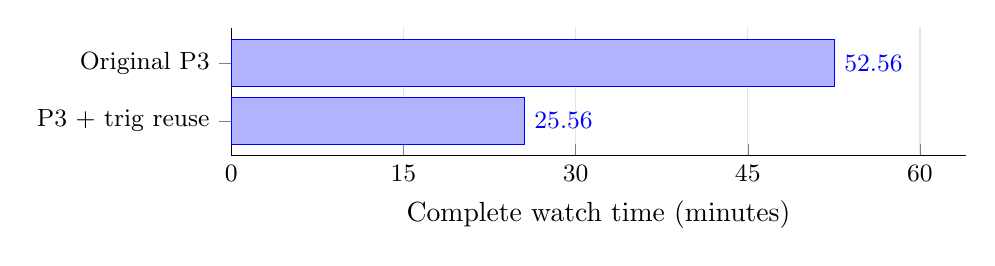
\begin{tikzpicture}
\begin{axis}[width=.9\linewidth,height=3.2cm,xbar,bar width=17pt,
xmin=0,xmax=64,ytick={1,2},yticklabels={P3 + trig reuse,Original P3},
ymin=.4,ymax=2.6,xtick={0,15,30,45,60},xlabel={Complete watch time (minutes)},
axis x line*=bottom,axis y line*=left,xmajorgrids=true,
grid style={gray!20},tick label style={font=\small},
nodes near coords,nodes near coords style={font=\small},
every axis plot/.append style={fill=teal,draw=teal}]
\addplot coordinates {(25.5625,1) (52.5575,2)};
\end{axis}\end{tikzpicture}\end{center}
{\footnotesize\setlength{\tabcolsep}{3.2pt}\renewcommand{\arraystretch}{1.18}
\noindent\begin{tabular*}{\linewidth}{@{\extracolsep{\fill}}lrrr@{}}\toprule
\textbf{Timing component} & \textbf{Original P3 s} & \textbf{Reuse P3 s} & \textbf{Original / new}\\ \midrule
Complete watch & 3153.449456 & 1533.752052 & 2.056\\
Cumulative advance & 2868.586754 & 1234.852041 & 2.323\\
Cumulative NN calls & 3.420546 & 3.533022 & 0.968\\
\bottomrule\end{tabular*}\par{}}\vspace{0.2cm}Same full 1000-step configuration: 51.36\% less time in one run, not a five-run benchmark timing.
\src{S06. Includes initialization, graph setup, logging, and checks; a native job was also running on other GPU/CPU resources.}
\end{frame}

% Slide 22
\begin{frame}[t]{QUAD speedup preserved every saved numerical output}
\relax
\relax
\begin{itemize}
\item \textbf{All 1000 observer files are identical.} They include endpoint/tube ranges, acceptance masks, and states for all 1024 partitions.
\item \textbf{All 50 controller, 50 transfer, and terminal files are identical.}
\item \textbf{Two final complete states match.} Plant, 14 SR/host components, progress, and final SR reset were checked.
\item The model, initial set, P3 orders, remainder cap, SR history, and 1000-step workload were retained.
\item Peak GPU memory was about 11.15 GiB and RSS about 5.63 GiB; GPU resource guard was 14 GiB.
\end{itemize}
\src{S06. Actual remote CPU data were checked and key JSON records archived locally; these provide evidence of output equivalence for the recorded runs.}
\end{frame}

% Slide 23
\begin{frame}[t]{QUAD at T=5: mode differences still matter}
\relax
\relax
{\small\setlength{\tabcolsep}{3.2pt}\renewcommand{\arraystretch}{1.18}
\noindent\begin{tabular*}{\linewidth}{@{\extracolsep{\fill}}lrr@{}}\toprule
\textbf{State} & \textbf{Huan parity global hull} & \textbf{Our P3 global hull}\\ \midrule
x1 & 6.4997094 & 6.6236214\\
x2 & 7.0530187 & 7.2535537\\
x3 & 0.047687232 & 0.068972382\\
x5 & 1.6005968 & 1.7220725\\
x6 & 0.12335096 & 0.1799271\\
x7 & 0.0070165625 & 0.01085314\\
\bottomrule\end{tabular*}\par{}}\vspace{0.3cm}Both complete to T=5, but parity and corrected P3 differ in order, error handling, and bounds.\par{}The new trig and original P3 have identical widths. Full T=5 values for Huan strict, Xiangru strict, and Flow* are still unavailable.
\src{S02, S05–S06. Absolute values are juxtaposed as observed; a narrower enclosure alone does not prove correct coverage.}
\end{frame}

% Slide 24
\begin{frame}[t]{QUAD versus the new native entry: common 40 steps}
\relax
\relax
{\footnotesize\setlength{\tabcolsep}{3.2pt}\renewcommand{\arraystretch}{1.18}
\noindent\begin{tabular*}{\linewidth}{@{\extracolsep{\fill}}lrrrr@{}}\toprule
\textbf{State} & \textbf{Our mean} & \textbf{Native mean} & \textbf{Our global hull} & \textbf{Native global hull}\\ \midrule
x1 & 0.1806475 & 0.1834987 & 0.960742 & 0.963601\\
x3 & 0.2144799 & 0.2165988 & 0.8208428 & 0.8229604\\
x5 & 0.8112718 & 0.8207659 & 0.8128924 & 0.8221873\\
x6 & 0.6027428 & 0.6030136 & 1.477771 & 1.478059\\
x7 & 0.00461459 & 0.004584761 & 0.005191669 & 0.005161935\\
\bottomrule\end{tabular*}\par{}}\vspace{0.35cm}At \(t=.2\), both accept all 1024 partitions on the same requested boxes / native-f64.\par{}Our method is P3; native is P2 with repaired initial coverage. Actual affine forms and subsequent NN domains need not match bitwise.\par{}Our/native observed 40-step process times are 155.452 / 171.138 s; diagnostic overhead differs, so no benchmark speedup is reported.
\src{S08, S10. Our time here is the pre-optimization P3 diagnostic, not the full trig-reuse time or a 40-step benchmark timing.}
\end{frame}

% Slide 25
\begin{frame}[t]{Native QUAD: initial-coverage repair and 400-step snapshot}
\relax
\relax
\begin{itemize}
\item On the same 8dd requested boxes, native initialization under-enclosed 384 lower endpoints across 338 partitions by 1 ULP.
\item An isolated variant retains the original center and library while taking the maximum outward distance as its radius; all 16,384 exact coverage checks pass.
\item After the repair, all 40 steps and two NN calls are accepted. Replays of the two actual NN inputs match 86,016 T/L/U floating-point outputs.
\item \textbf{Last saved snapshot: 400/1000 steps; all 1024 partitions accepted.} Timestamp: September 29, 20:19:53 China time. No terminal state is available.
\item Host-memory budget: 128 GiB; GPU guard: 14 GiB; four CPU workers. No complete T=5 time or width is available.
\end{itemize}
\src{S10. This report reads a local saved snapshot without reconnecting to the server; 400 steps is not a live status.}
\end{frame}

% Slide 26
\begin{frame}[t]{What the correctness checks support}
\relax
\relax
{\footnotesize\renewcommand{\arraystretch}{1.12}\noindent\begin{tabularx}{\linewidth}{@{}X X@{}}\toprule
\textbf{Evidence obtained} & \textbf{Still outside its scope}\\\midrule
Exact initial-set inclusion; replayed interface ordering and dtype. & End-to-end proof of controller FP bounds and RN injections.\\
Cold resume; accepted steps and partitions; numerical and SR component comparisons. & All inputs, combinations of operations, and future trajectories.\\
ACC analytic counterexample and isolated fix; generic reciprocal counterexamples located. & Generic counterexamples do not prove lost trajectories in every benchmark.\\
Parameters, resource changes, failures, and incomplete runs recorded. & Suite regression and five timed runs for the new QUAD candidate.\\
\bottomrule\end{tabularx}\par{}}\vspace{0.3cm}No evidence of reduced work, discarded required error, or hidden rejections.\par{}A ``strict'' switch, VERIFIED log, or similar width does not prove end-to-end correctness.
\src{S01, S04, S06, S10, S12–S13.}
\end{frame}

% Slide 27
\begin{frame}[t]{Current progress and next priorities}
\relax
\relax
{\small\renewcommand{\arraystretch}{1.18}\noindent\begin{tabularx}{\linewidth}{@{}X X@{}}\toprule
\textbf{Established so far} & \textbf{To complete later}\\\midrule
Four-way screening of 14 configurations; seven cases with five timed runs per method. & Rerun affected regressions for new corrected revisions, rather than inherit older results.\\
Complete P3 QUAD; same outputs in roughly half the total time. & Match modes for Huan/Xiangru and complete native T=5; then repeat timing.\\
Airplane with actual NN calls and an explained stop at step 78. & Huan/Xiangru metadata-resource issue and cost under a common stop contract.\\
Corrected ACC reference and narrowed localization of Unicycle width gap. & General regression of the repaired reference, remaining tube gap, and Unicycle internal attribution.\\
\bottomrule\end{tabularx}\par{}}\vspace{0.45cm}\textbf{This presentation summarizes saved experiments only; the experimental task remains paused.}
\src{Numbers are current through the saved evidence; the listed future work has not yet been carried out.}
\end{frame}

% Slide 28
\begin{frame}[t]{Appendix: Attempts without four complete results}
\relax
\relax
{\footnotesize\setlength{\tabcolsep}{3.2pt}\renewcommand{\arraystretch}{1.18}
\noindent\begin{tabular*}{\linewidth}{@{\extracolsep{\fill}}lrrrr@{}}\toprule
\textbf{Case} & \textbf{Ours} & \textbf{Huan} & \textbf{Xiangru} & \textbf{Native Flow*}\\ \midrule
DP more robust & early stop 5.36 & early stop 5.63 & early stop 5.76 & early stop 5.11\\
DP less robust & complete 8.76 & complete 8.30 & complete 8.51 & timeout 303.66\\
NAV standard & complete 14.15 & complete 18.12 & complete 17.91 & timeout 303.93\\
CartPole & rejected 12.65 & rejected 13.77 & rejected 13.99 & numeric stop 8.94\\
TORA homogeneous & complete 7.88 & rejected 8.90 & rejected 8.82 & complete 8.20\\
QUAD & rejected 35.81 & rejected 58.76 & rejected 61.56 & RSS stop 845.82\\
\bottomrule\end{tabular*}\par{}}\vspace{0.15cm}Seconds; one observer-instrumented run per method; separate from five-run medians.\par{}QUAD uses the initial ARCH contract; later variants are labeled. See Airplane in the main slides.\par{}DP more robust actually loaded the less robust model; both labels are recorded.
\src{S01. Full step counts, outcomes, and resources: arch\_diagnostic\_attempts.csv.}
\end{frame}

% Slide 29
\begin{frame}[t]{Appendix: Official benchmark settings (1/2)}
\relax
\relax
{\footnotesize\setlength{\tabcolsep}{3.2pt}\renewcommand{\arraystretch}{1.18}
\noindent\begin{tabular*}{\linewidth}{@{\extracolsep{\fill}}lrrrrrr@{}}\toprule
\textbf{Case} & \textbf{B} & \textbf{h / order} & \textbf{ctrl. \(\times\) N} & \textbf{T} & \textbf{steps} & \textbf{rem.}\\ \midrule
Attitude & 1 & 0.05/3 & 0.1\(\times\)30 & 3 & 60 & \(\pm0.01\)\\
DP more robust & 1 & 0.005/4 & 0.02\(\times\)20 & 0.4 & 80 & \(\pm0.01\)\\
DP less robust & 225 & 0.01/4 & 0.05\(\times\)20 & 1 & 100 & \(\pm0.01\)\\
NAV robust & 25 & 0.01/4 & 0.2\(\times\)30 & 6 & 600 & \(\pm0.1\)\\
NAV standard & 640 & 0.01/4 & 0.2\(\times\)30 & 6 & 600 & \(\pm0.1\)\\
Unicycle & 1 & 0.02/2 & 0.2\(\times\)50 & 10 & 500 & \(\pm0.01\)\\
TORA ReLU/tanh & 1 & 0.01/6 & 0.5\(\times\)10 & 5 & 500 & \(\pm0.01\)\\
\bottomrule\end{tabular*}\par{}}\vspace{0.3cm}Cutoff \(10^{-6}\); default SR 1000, except ACC at 50. Unicycle also has disturbance \(w\in[-10^{-4},10^{-4}]\). B is the number of initial boxes.\par{}This is the historical ARCH contract. The current QUAD P3 order and native-f64 variant are specified separately.
\src{S01. Exact initial boxes, splits, model/box hashes, and configuration files: data/arch\_configurations.csv.}
\end{frame}

% Slide 30
\begin{frame}[t]{Appendix: Official benchmark settings (2/2)}
\relax
\relax
{\footnotesize\setlength{\tabcolsep}{3.2pt}\renewcommand{\arraystretch}{1.18}
\noindent\begin{tabular*}{\linewidth}{@{\extracolsep{\fill}}lrrrrrr@{}}\toprule
\textbf{Case} & \textbf{B} & \textbf{h / order} & \textbf{ctrl. \(\times\) N} & \textbf{T} & \textbf{steps} & \textbf{rem.}\\ \midrule
TORA sigmoid & 1 & 0.01/6 & 0.5\(\times\)10 & 5 & 500 & \(\pm0.01\)\\
CartPole & 1 & 0.005/6 & 0.02\(\times\)50 & 1 & 200 & \(\pm0.1\)\\
Airplane & 1 & 0.01/6 & 0.1\(\times\)20 & 2 & 200 & \(\pm0.01\)\\
Single Pendulum & 1 & 0.01/2 & 0.05\(\times\)20 & 1 & 100 & \(\pm0.01\)\\
TORA homogeneous & 12 & 0.1/3 & 1.0\(\times\)20 & 20 & 200 & \(\pm0.01\)\\
ACC* & 1 & 0.1/3 & 0.1\(\times\)50 & 5 & 50 & \(\pm0.1\)\\
QUAD & 1024 & 0.005/2 & 0.1\(\times\)50 & 5 & 1000 & \(\pm0.1\)\\
\bottomrule\end{tabular*}\par{}}\vspace{0.3cm}Cutoff \(10^{-6}\); default SR 1000, except ACC at 50. Unicycle also has disturbance \(w\in[-10^{-4},10^{-4}]\). B is the number of initial boxes.\par{}This is the historical ARCH contract. The current QUAD P3 order and native-f64 variant are specified separately.
\src{S01. Exact initial boxes, splits, model/box hashes, and configuration files: data/arch\_configurations.csv.}
\end{frame}

% Slide 31
\begin{frame}[t]{Appendix: Runtime sample ranges (1/2)}
\relax
\relax
{\scriptsize\setlength{\tabcolsep}{3.2pt}\renewcommand{\arraystretch}{1.18}
\noindent\begin{tabular*}{\linewidth}{@{\extracolsep{\fill}}lrrrr@{}}\toprule
\textbf{Case} & \textbf{Ours} & \textbf{Huan} & \textbf{Xiangru} & \textbf{Flow*}\\ \midrule
Attitude & 7.121 [6.979, 7.186] & 6.990 [6.960, 7.059] & 7.028 [6.839, 7.376] & 6.315 [6.111, 6.355]\\
Unicycle & 6.909 [6.852, 7.042] & 9.796 [9.622, 10.058] & 9.581 [9.544, 10.054] & 10.722 [10.554, 10.778]\\
TORA ReLU/tanh & 7.685 [7.659, 7.875] & 12.421 [12.137, 12.503] & 12.332 [12.226, 12.705] & 8.632 [8.617, 8.676]\\
TORA sigmoid & 8.208 [8.127, 8.310] & 13.165 [12.969, 13.259] & 13.274 [13.188, 13.515] & 9.098 [9.034, 9.121]\\
\bottomrule\end{tabular*}\par{}}\vspace{0.4cm}Each cell gives median [min, max] in seconds across five runs.\par{}V100 GPU 3 and CPUs 14–17 were fixed; runs were interleaved and each group's first warmup was excluded. The node was shared.
\src{S01. The 140 counted runs and 28 excluded warmups: arch\_timing\_samples.csv; see main slides for the ACC correction.}
\end{frame}

% Slide 32
\begin{frame}[t]{Appendix: Runtime sample ranges (2/2)}
\relax
\relax
{\scriptsize\setlength{\tabcolsep}{3.2pt}\renewcommand{\arraystretch}{1.18}
\noindent\begin{tabular*}{\linewidth}{@{\extracolsep{\fill}}lrrrr@{}}\toprule
\textbf{Case} & \textbf{Ours} & \textbf{Huan} & \textbf{Xiangru} & \textbf{Flow*}\\ \midrule
NAV robust & 9.730 [9.349, 9.967] & 14.646 [14.071, 15.074] & 14.814 [14.045, 14.916] & 68.164 [66.916, 78.318]\\
Single Pendulum & 5.176 [5.068, 5.375] & 5.597 [5.527, 5.624] & 5.618 [5.504, 5.819] & 4.908 [4.773, 4.917]\\
ACC* & 7.793 [7.740, 7.868] & 8.035 [7.876, 8.078] & 7.960 [7.862, 8.081] & 8.259 [8.224, 8.342]\\
\bottomrule\end{tabular*}\par{}}\vspace{0.4cm}Each cell gives median [min, max] in seconds across five runs.\par{}V100 GPU 3 and CPUs 14–17 were fixed; runs were interleaved and each group's first warmup was excluded. The node was shared.
\src{S01. The 140 counted runs and 28 excluded warmups: arch\_timing\_samples.csv; see main slides for the ACC correction.}
\end{frame}

% Slide 33
\begin{frame}[t]{Appendix: Endpoint widths — Attitude and Pendulum}
\relax
\relax
{\footnotesize\setlength{\tabcolsep}{3.2pt}\renewcommand{\arraystretch}{1.18}
\noindent\begin{tabular*}{\linewidth}{@{\extracolsep{\fill}}lrrrr@{}}\toprule
\textbf{State} & \textbf{Flow*} & \textbf{Huan} & \textbf{Xiangru} & \textbf{Ours}\\ \midrule
Attitude \(x_1\) & 0.004194134 & 0.004174214 & 0.004174214 & 0.004398305\\
Attitude \(x_2\) & 0.005980154 & 0.005935659 & 0.005935659 & 0.006299372\\
Attitude \(x_3\) & 0.006193977 & 0.006172913 & 0.006172913 & 0.006555204\\
Attitude \(x_4\) & 0.03229213 & 0.03207033 & 0.03207033 & 0.03384848\\
Attitude \(x_5\) & 0.01763594 & 0.01736152 & 0.01736152 & 0.01848375\\
Attitude \(x_6\) & 0.0186374 & 0.01847936 & 0.01847936 & 0.01971919\\
Single Pendulum \(x_1\) & 0.1391394 & 0.1482617 & 0.1482617 & 0.1438742\\
Single Pendulum \(x_2\) & 0.1444355 & 0.1551737 & 0.1551737 & 0.1502648\\
\bottomrule\end{tabular*}\par{}}\vspace{0.25cm}Endpoint width of the global hull at the final time; state units follow each model.
\src{S01. CSV retains full precision and per-state statistics over time; see S04 for the corrected ACC reference.}
\end{frame}

% Slide 34
\begin{frame}[t]{Appendix: Endpoint widths — two heterogeneous TORA cases}
\relax
\relax
{\footnotesize\setlength{\tabcolsep}{3.2pt}\renewcommand{\arraystretch}{1.18}
\noindent\begin{tabular*}{\linewidth}{@{\extracolsep{\fill}}lrrrr@{}}\toprule
\textbf{State} & \textbf{Flow*} & \textbf{Huan} & \textbf{Xiangru} & \textbf{Ours}\\ \midrule
TORA ReLU/tanh \(x_1\) & 0.02512807 & 0.02507951 & 0.02507951 & 0.02509966\\
TORA ReLU/tanh \(x_2\) & 0.02745754 & 0.02741052 & 0.02741052 & 0.02739115\\
TORA ReLU/tanh \(x_3\) & 0.02203482 & 0.02199292 & 0.02199292 & 0.02201384\\
TORA ReLU/tanh \(x_4\) & 0.02161695 & 0.02159111 & 0.02159111 & 0.02165234\\
TORA sigmoid \(x_1\) & 0.02487467 & 0.02480363 & 0.02480363 & 0.02489772\\
TORA sigmoid \(x_2\) & 0.02635339 & 0.02628228 & 0.02628228 & 0.02628759\\
TORA sigmoid \(x_3\) & 0.02610609 & 0.02602511 & 0.02602511 & 0.02608528\\
TORA sigmoid \(x_4\) & 0.02799618 & 0.02794208 & 0.02794208 & 0.02804373\\
\bottomrule\end{tabular*}\par{}}\vspace{0.25cm}Endpoint width of the global hull at the final time; state units follow each model.
\src{S01. CSV retains full precision and per-state statistics over time; see S04 for the corrected ACC reference.}
\end{frame}

% Slide 35
\begin{frame}[t]{Appendix: Endpoint widths — NAV robust and Unicycle}
\relax
\relax
{\footnotesize\setlength{\tabcolsep}{3.2pt}\renewcommand{\arraystretch}{1.18}
\noindent\begin{tabular*}{\linewidth}{@{\extracolsep{\fill}}lrrrr@{}}\toprule
\textbf{State} & \textbf{Flow*} & \textbf{Huan} & \textbf{Xiangru} & \textbf{Ours}\\ \midrule
NAV robust \(x_1\) & 0.0909985 & 0.09030302 & 0.09030302 & 0.09134372\\
NAV robust \(x_2\) & 0.01507649 & 0.01480299 & 0.01480299 & 0.01511633\\
NAV robust \(x_3\) & 0.02489178 & 0.02461458 & 0.02461458 & 0.02495127\\
NAV robust \(x_4\) & 0.2941089 & 0.2924141 & 0.2924141 & 0.294786\\
Unicycle \(x_1\) & 0.04038534 & 0.09540937 & 0.09540937 & 0.09669186\\
Unicycle \(x_2\) & 0.06082288 & 0.1409442 & 0.1409442 & 0.1428876\\
Unicycle \(x_3\) & 0.04165892 & 0.1313937 & 0.1313937 & 0.1337685\\
Unicycle \(x_4\) & 0.03520954 & 0.1212424 & 0.1212424 & 0.123212\\
\bottomrule\end{tabular*}\par{}}\vspace{0.25cm}Endpoint width of the global hull at the final time; state units follow each model.
\src{S01. CSV retains full precision and per-state statistics over time; see S04 for the corrected ACC reference.}
\end{frame}

% Slide 36
\begin{frame}[t]{Appendix: Endpoint widths — historical ACC output}
\relax
\relax
{\footnotesize\setlength{\tabcolsep}{3.2pt}\renewcommand{\arraystretch}{1.18}
\noindent\begin{tabular*}{\linewidth}{@{\extracolsep{\fill}}lrrrr@{}}\toprule
\textbf{State} & \textbf{Flow*} & \textbf{Huan} & \textbf{Xiangru} & \textbf{Ours}\\ \midrule
ACC* \(x_1\) & 20.99393 & 21.01204 & 21.01204 & 21.01046\\
ACC* \(x_2\) & 0.1975723 & 0.2017539 & 0.2017539 & 0.2016287\\
ACC* \(x_3\) & 0.0006846514 & 0.0007410763 & 0.0007410763 & 0.0007376998\\
ACC* \(x_4\) & 5.028369 & 5.497976 & 5.497976 & 5.333353\\
ACC* \(x_5\) & 1.795632 & 2.015511 & 2.015511 & 1.948656\\
ACC* \(x_6\) & 1.0637 & 1.181106 & 1.181106 & 1.15943\\
\bottomrule\end{tabular*}\par{}}\vspace{0.25cm}Endpoint width of the global hull at the final time; state units follow the model.\par{} The historical native ACC result omitted reachable states. This table preserves its output and is not a valid accuracy reference.
\src{S01. CSV retains full precision and per-state statistics over time; see S04 for the corrected ACC reference.}
\end{frame}

% Slide 37
\begin{frame}[t]{Appendix: QUAD widths at T=5, states 1–6}
\relax
\relax
{\footnotesize\setlength{\tabcolsep}{3.2pt}\renewcommand{\arraystretch}{1.18}
\noindent\begin{tabular*}{\linewidth}{@{\extracolsep{\fill}}lrrrr@{}}\toprule
\textbf{State} & \textbf{P3 mean} & \textbf{P3 max} & \textbf{P3 hull} & \textbf{Huan parity hull}\\ \midrule
x1 & 3.8904615 & 3.9143939 & 6.6236214 & 6.4997094\\
x2 & 6.5097634 & 6.5323884 & 7.2535537 & 7.0530187\\
x3 & 0.062617019 & 0.064438385 & 0.068972382 & 0.047687232\\
x4 & 1.090248 & 1.1008754 & 1.5039563 & 1.4226317\\
x5 & 1.7028656 & 1.7126352 & 1.7220725 & 1.6005968\\
x6 & 0.1679 & 0.17312141 & 0.1799271 & 0.12335096\\
\bottomrule\end{tabular*}\par{}}\vspace{0.3cm}Original P3 and the trig-reuse version have identical saved numbers. Huan parity and P3 use different error and order settings.\par{}x12 is constant; P3's roughly \(4.45\times10^{-308}\) is roundoff noise, so no ratio is reported.
\src{S02, S05–S06. Complete T=5 widths are unavailable for strict Huan, strict Xiangru, and Flow*; no values were imputed.}
\end{frame}

% Slide 38
\begin{frame}[t]{Appendix: QUAD widths at T=5, states 7–12}
\relax
\relax
{\footnotesize\setlength{\tabcolsep}{3.2pt}\renewcommand{\arraystretch}{1.18}
\noindent\begin{tabular*}{\linewidth}{@{\extracolsep{\fill}}lrrrr@{}}\toprule
\textbf{State} & \textbf{P3 mean} & \textbf{P3 max} & \textbf{P3 hull} & \textbf{Huan parity hull}\\ \midrule
x7 & 0.010151003 & 0.010497058 & 0.01085314 & 0.0070165625\\
x8 & 0.0092057392 & 0.0095347946 & 0.0097108278 & 0.0061199043\\
x9 & 0.0060247288 & 0.0061434876 & 0.0061434876 & 0.0044494068\\
x10 & 0.14977017 & 0.15565646 & 0.15565646 & 0.086179577\\
x11 & 0.12566507 & 0.13084117 & 0.13084117 & 0.071020671\\
x12 & \(4.4501477\times10^{-308}\) & \(4.4501477\times10^{-308}\) & \(4.4501477\times10^{-308}\) & 0\\
\bottomrule\end{tabular*}\par{}}\vspace{0.3cm}Original P3 and the trig-reuse version have identical saved numbers. Huan parity and P3 use different error and order settings.\par{}x12 is constant; P3's roughly \(4.45\times10^{-308}\) is roundoff noise, so no ratio is reported.
\src{S02, S05–S06. Complete T=5 widths are unavailable for strict Huan, strict Xiangru, and Flow*; no values were imputed.}
\end{frame}

% Slide 39
\begin{frame}[t]{Appendix: QUAD four-way reference at t=0.5, states 1–6}
\relax
\relax
{\footnotesize\setlength{\tabcolsep}{3.2pt}\renewcommand{\arraystretch}{1.18}
\noindent\begin{tabular*}{\linewidth}{@{\extracolsep{\fill}}lrrrrr@{}}\toprule
\textbf{State} & \textbf{Our P3} & \textbf{Our P2} & \textbf{Huan} & \textbf{Xiangru} & \textbf{Flow*}\\ \midrule
x1 & 1.209483 & 1.210965 & 1.212697 & 1.212697 & 1.215011\\
x2 & 1.208691 & 1.211738 & 1.216197 & 1.216197 & 1.21431\\
x3 & 0.4934754 & 0.4983923 & 0.5015186 & 0.5015186 & 0.4962256\\
x4 & 0.8259578 & 0.8302554 & 0.8346602 & 0.8346602 & 0.8348579\\
x5 & 0.8578122 & 0.8743562 & 0.8928963 & 0.8928963 & 0.8676566\\
x6 & 1.526041 & 1.533748 & 1.538956 & 1.538956 & 1.529488\\
\bottomrule\end{tabular*}\par{}}\vspace{0.35cm}Endpoint global hull for the common valid prefix of 100 steps.\par{}The three ARCH runs use f90 initial boxes / RPC32. Our P2/P3 use 8dd / native-f64, with different orders.\par{}This is a descriptive reference with contract differences, not a strict same-input algorithm ranking.
\src{S09. The named CSV and RESULT files give all state widths, contract differences, and provenance.}
\end{frame}

% Slide 40
\begin{frame}[t]{Appendix: QUAD four-way reference at t=0.5, states 7–11}
\relax
\relax
{\footnotesize\setlength{\tabcolsep}{3.2pt}\renewcommand{\arraystretch}{1.18}
\noindent\begin{tabular*}{\linewidth}{@{\extracolsep{\fill}}lrrrrr@{}}\toprule
\textbf{State} & \textbf{Our P3} & \textbf{Our P2} & \textbf{Huan} & \textbf{Xiangru} & \textbf{Flow*}\\ \midrule
x7 & 0.01237843 & 0.01484585 & 0.01747069 & 0.01747069 & 0.01240678\\
x8 & 0.01166923 & 0.01405786 & 0.0165278 & 0.0165278 & 0.01170151\\
x9 & 0.0001417913 & 0.0001689534 & 0.0002153181 & 0.0002153181 & 0.0001298099\\
x10 & 0.2100149 & 0.2139019 & 0.2186553 & 0.2186553 & 0.2102979\\
x11 & 0.1978412 & 0.2015494 & 0.2059809 & 0.2059809 & 0.1981034\\
\bottomrule\end{tabular*}\par{}}\vspace{0.35cm}Endpoint global hull for the common valid prefix of 100 steps.\par{}The three ARCH runs use f90 initial boxes / RPC32. Our P2/P3 use 8dd / native-f64, with different orders.\par{}This is a descriptive reference with contract differences, not a strict same-input algorithm ranking.
\src{S09. The named CSV and RESULT files give all state widths, contract differences, and provenance.}
\end{frame}

% Slide 41
\begin{frame}[t]{Appendix: Fixed-plant baselines reported previously}
\relax
\relax
{\small\setlength{\tabcolsep}{3.2pt}\renewcommand{\arraystretch}{1.18}
\noindent\begin{tabular*}{\linewidth}{@{\extracolsep{\fill}}lrrrr@{}}\toprule
\textbf{Case} & \textbf{Ours} & \textbf{Huan} & \textbf{Xiangru} & \textbf{Flow*}\\ \midrule
Van der Pol B1 & 2.921487 & 12.552073 & 12.602979 & 1.447977\\
Van der Pol B32 & 0.769654 & 0.840225 & 0.837461 & 0.682880\\
Brusselator B1 & 4.456490 & 16.867330 & 16.737087 & 13.847315\\
Brusselator B32 & 0.897973 & 0.929344 & 0.935446 & 8.053289\\
\bottomrule\end{tabular*}\par{}}\vspace{0.35cm}These are five-run medians of core execution time from the previous slides; they were not rerun here.\par{}Core time excludes new-process startup and separate export. It cannot be ranked directly against the new NNCS process wall time.
\src{S00. Original VDP with one box remains slower than native Flow*; current work centers on official NNCS cases and QUAD.}
\end{frame}

% Slide 42
\begin{frame}[t]{Appendix: Evidence index and version scope}
\relax
\relax
{\small\renewcommand{\arraystretch}{1.18}\noindent\begin{tabularx}{\linewidth}{@{}p{3.5cm}X@{}}\toprule
\textbf{Source ID} & \textbf{Contents}\\\midrule
S00 / S01 & Prior slides/README; 14-case report, timings, widths, settings.\\
S02 / S03 & Huan QUAD parity/strict runs; corrected P2 to step 799.\\
S04 / S05 & ACC counterexample/fix; full P3 and step-799 comparison.\\
S06 & Full 1000-step trig run; INPUT/RESULT/COMMAND; CPU audit.\\
S07 / S08 / S09 & QUAD widths at steps 580, 40, 100.\\
S10 / S11 / S12 / S13 & Native coverage/snapshot; Airplane; Unicycle; operations/failures.\\
\bottomrule\end{tabularx}\par{}}\vspace{0.1cm}SOURCES.json maps original and copied paths with SHA-256 hashes.\par{}Missing results remain blank or have an explicit status.
\src{Sources and URLs: SOURCES.md. Large PT/SR files, weights, and environments remain on the server.}
\end{frame}
\end{document}
